\chapter{Results}

\section{Performance}

\subsection{Measurements}

Our setup for the performance tests was a PC with a Ryzen 7 3700X CPU and a Radeon RX 590 GPU.

See Table \ref{table:resultFPS}, See Figure \ref{fig:performanceNodes}, See Figure \ref{fig:performanceLinks}

Notes:
With an increasing number of links the variance of FPS increase. During the animated teleportation the FPS drop noticeably. We assume this is because of the often applied scaling to all entities in the scene. Filtering links does not influence performance. The maximum of 90 FPS is due to the 90HZ panel of the HTC Vive.
CPU and GPU utilization was only about 50\%

\begin{table}
    \centering
    \begin{tabular}{ | c | c | c | c | c | c | }
        \hline
        \textbf{nodes} & \textbf{links} &\textbf{layers} &\textbf{layout - FPS} &\textbf{expl. - min FPS} &\textbf{expl. - avg FPS}\\
        \hline
        310  & 0    & 3 & 40 & 90 & 90\\ \hline
        730  & 0    & 3 & 30 & 70 & 75\\ \hline
        1100 & 0    & 3 & 20 & 55 & 60\\ \hline
        1560 & 0    & 4 & 20 & 40 & 55\\ \hline
        2343 & 0    & 5 & 10 & 30 & 35\\ \hline
        774  & 387  & 3 & 20 & 60 & 70\\ \hline
        774  & 1548 & 3 & 20 & 55 & 70\\ \hline
        774  & 3870 & 3 & 10 & 40 & 60\\ \hline
        1560 & 3120 & 4 & 5  & 25 & 45\\ \hline
        1020 & 2040 & 4 & 10 & 40 & 60\\ \hline
     \end{tabular}
     \caption{Results from performance measurement evaluation(expl. ... exploration).}
     \label{table:resultFPS}
\end{table}


\begin{figure}[h]
    \centering
    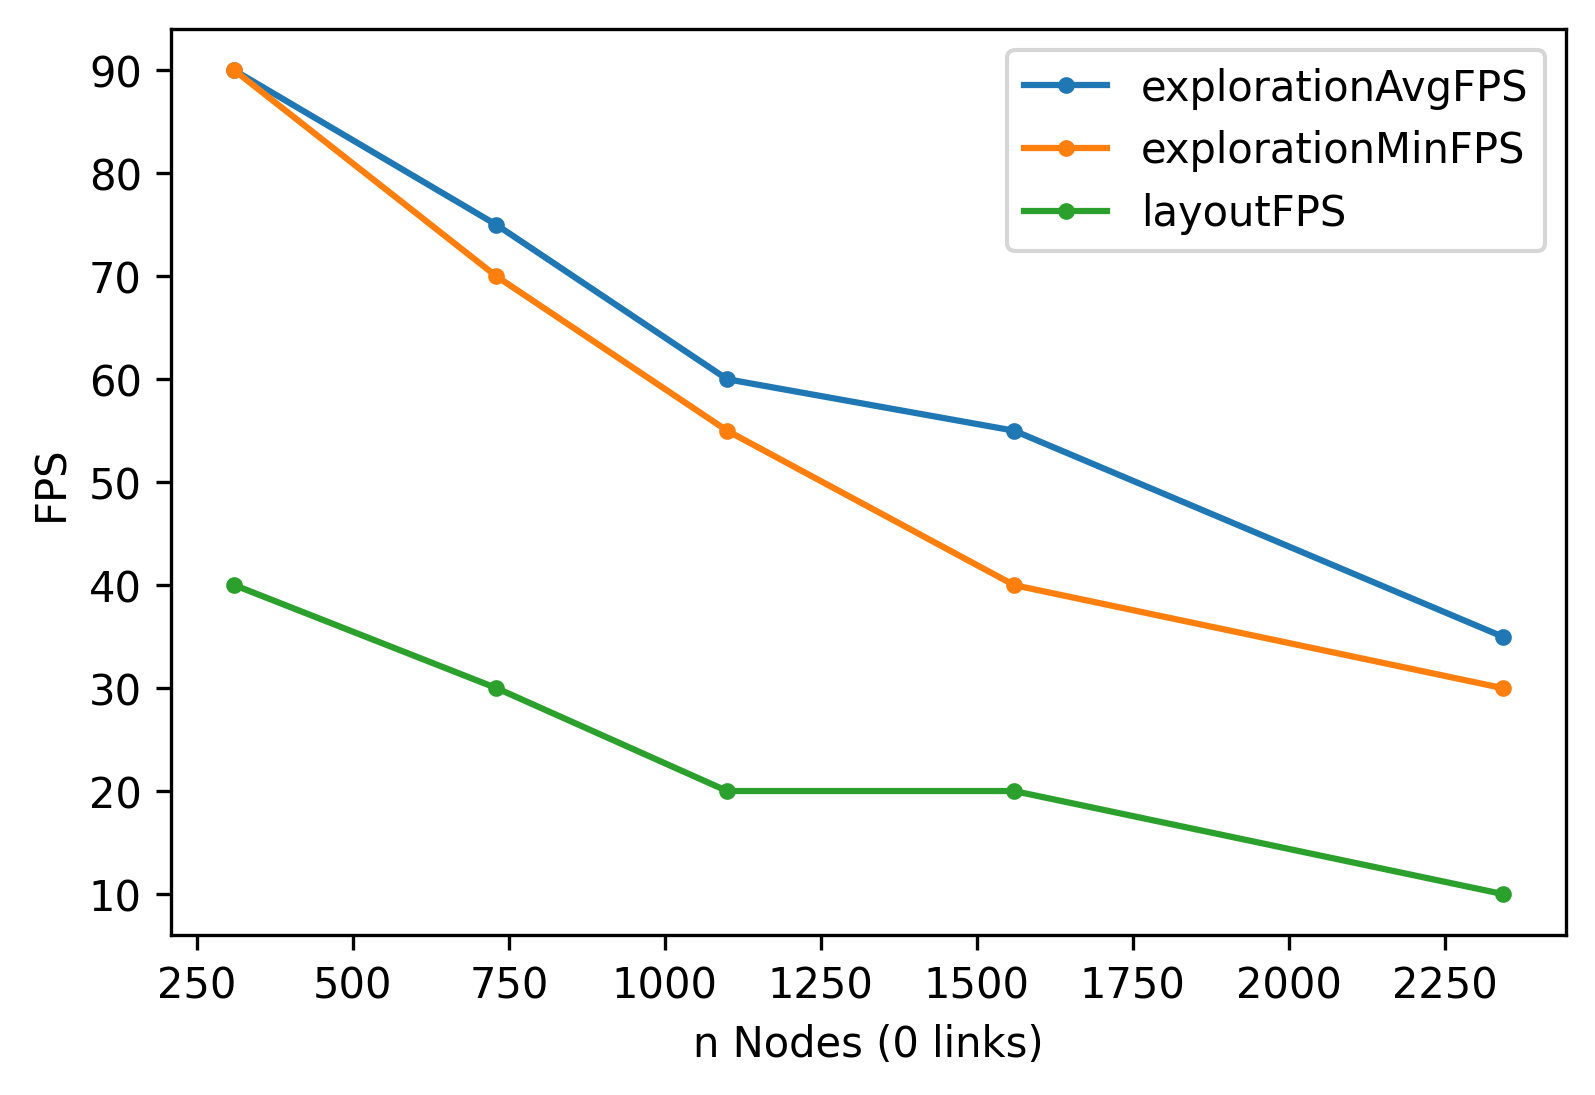
\includegraphics[width=0.75\textwidth]{graphics/performanceAnalysisNodes.png}
    \caption{Performance chart for scaling the number of nodes.} 
    \label{fig:performanceNodes} 
\end{figure}

\begin{figure}[h]
    \centering
    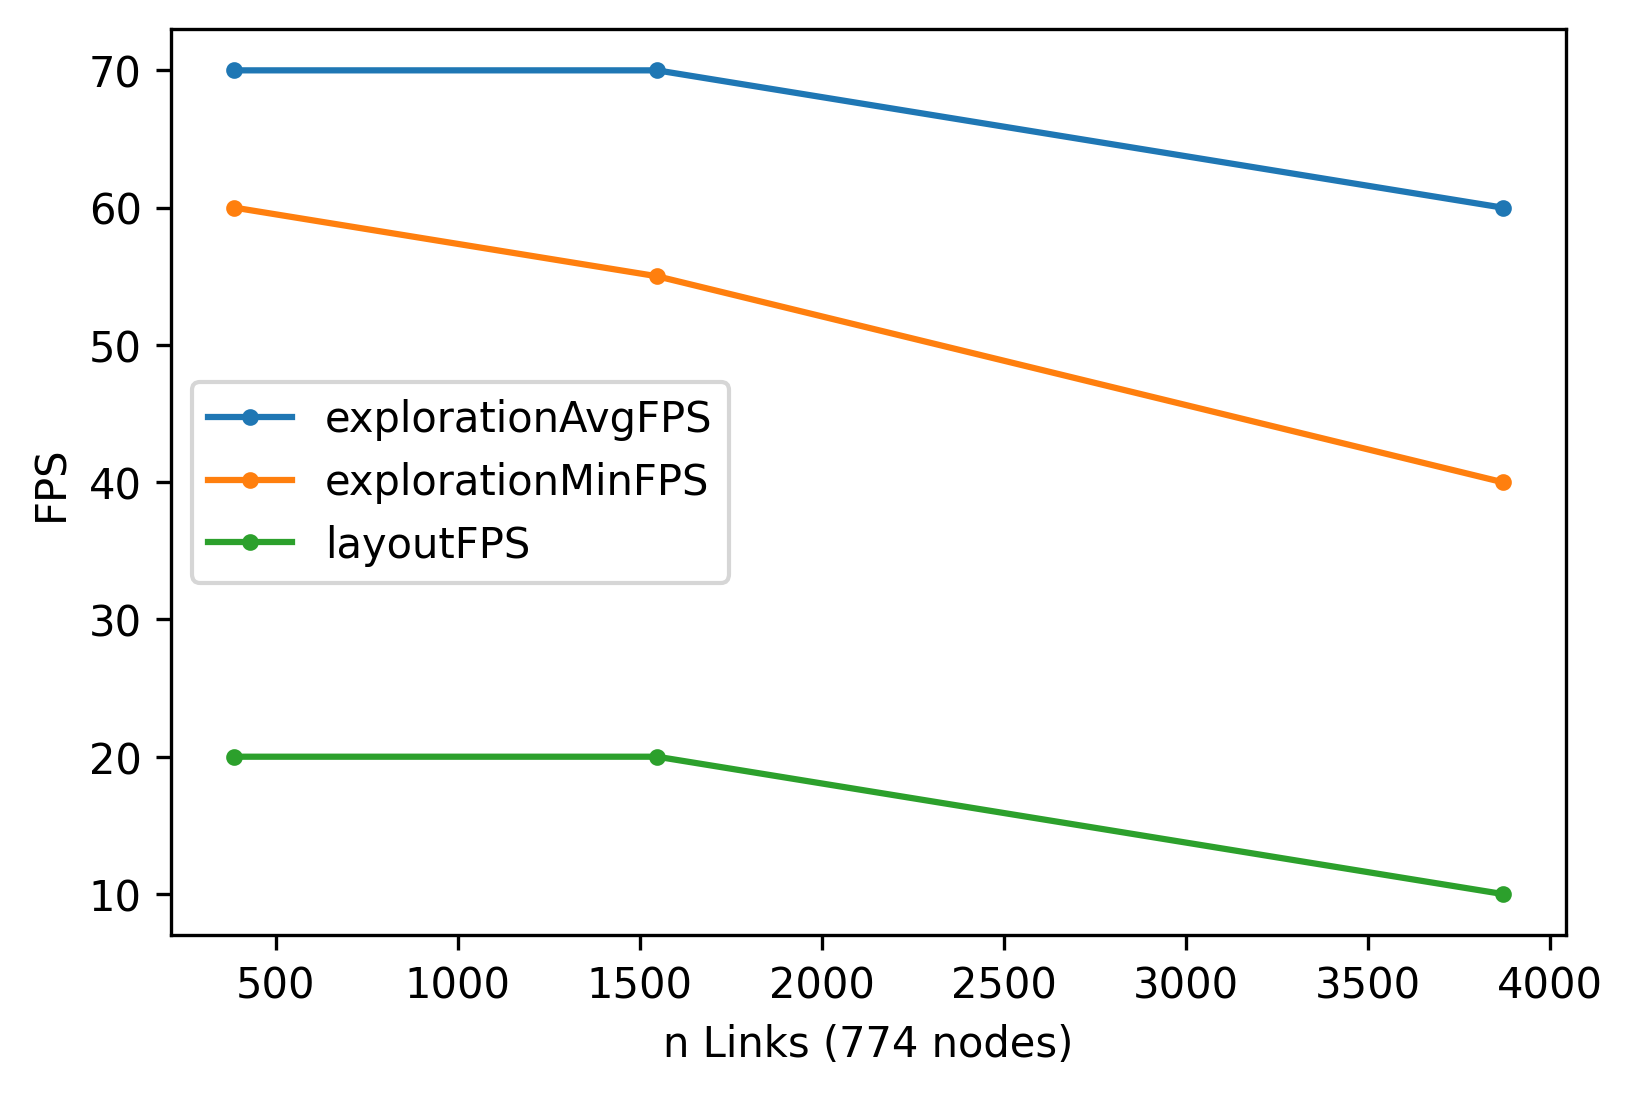
\includegraphics[width=0.75\textwidth]{graphics/performanceAnalysisLinks.png}
    \caption{Performance chart for scaling the number of links.} 
    \label{fig:performanceLinks} 
\end{figure}

\subsection{Possible optimization}

Raycasting only while a button is pressed. 

\section{Informal feedback}

\subsection{Clarity of the visualization}
Filtering, visual clutter, hierarchical layout(intuitive?), ...

\subsection{Navigation}
Free fly, animated teleport, scaling, motion sickness.

\subsection{Interaction}
Button Mappings, Laser Pointer, 

\subsection{Performance}
Tested system and dataset